% Romer (2012), Problem 6.7 (p. 308): solution only, the statement is not reproduced (CLAUDE.md).
% Every formula and number below is re-checked by check-6-10-6-7.py in this folder.
\problema{Romer 6.7}{The liquidity trap}{p.~308}{Romer \S6.4; Benigno (2015) \S9}

\noindent With $\bar y\equiv0$, $y$ is the output gap, $i$ the nominal rate and $i-\pi$ the real rate in the
traditional IS curve. The rule (6.26) is a continuously differentiable $r(y,\pi)$ with $r_1>0$ and
$r_2>0$. Two regularity conditions, both true for the linear rule used below, are assumed: for every
$\pi$ the equation $\theta y+r(y,\pi)=0$ has a solution, and the kink $(\tilde y,\tilde\pi)$ exists (the
statement presupposes it). The figures use $r=c+ay+b\pi$ with $\theta=2$, $a=1$, $b=3$, $\lambda=\frac12$,
and $c=-9$ (then $\tilde y>0$) or $c=4.5$ (then $\tilde y<0$); every result is proved for a general $r$.

\parte{a}
\passo{Combine the IS curve and the constrained rule}{The IS curve says $\theta y=\pi-i$. Substituting $i=\max[0,\pi+r(y,\pi)]$ and using $-\max\{u,v\}=\min\{-u,-v\}$,
\[ \theta y=\pi-\max\bigl[0,\ \pi+r(y,\pi)\bigr]=\min\bigl[\pi,\ -r(y,\pi)\bigr]. \]
This single equation is the AD curve. Equivalently, the real rate is $i-\pi=\max[r(y,\pi),-\pi]$: what the bank wants, unless that lies below the floor $-\pi$ imposed by $i\ge0$.}
\passo{The two branches}{A minimum equals $\theta y$ iff one term equals $\theta y$ and the other is not smaller, so a point is on the AD curve iff
\[ \begin{aligned} &\text{(L), zero bound binding:} && \theta y=\pi && \text{and} && \pi+r(y,\pi)\le0,\\ &\text{(U), zero bound slack:} && \theta y+r(y,\pi)=0 && \text{and} && \pi+r(y,\pi)\ge0 . \end{aligned} \]
At the kink both hold: $\theta\tilde y=\tilde\pi$ and $\theta\tilde y+r(\tilde y,\tilde\pi)=0$.}
\passo{Which branch applies where}{On the line $\pi=\theta y$ let $h(y)\equiv\theta y+r(y,\theta y)$; then $h'(y)=\theta+r_1+\theta r_2>0$ and $h(\tilde y)=0$, so a point of the line is on (L) iff $h(y)\le0$, i.e.\ iff $y\le\tilde y$, i.e.\ iff $\pi\le\tilde\pi$. On (U), $y=Y(\pi)$, the unique root of $\theta y+r(y,\pi)=0$ (its left side rises in $y$ at rate $\theta+r_1>0$), with $Y(\tilde\pi)=\tilde y$ and, by implicit differentiation, $Y'(\pi)=-r_2/(\theta+r_1)<0$. Since $r(Y,\pi)=-\theta Y$, the side condition of (U) is $k(\pi)\equiv\pi-\theta Y(\pi)\ge0$; as $k'(\pi)=1+\theta r_2/(\theta+r_1)>0$ and $k(\tilde\pi)=0$, it holds iff $\pi\ge\tilde\pi$. Hence each $\pi$ has exactly one output level on the AD curve:
\[ y=A(\pi)\equiv\begin{cases} \pi/\theta, & \pi\le\tilde\pi\quad\text{(nominal rate at zero)},\\ Y(\pi), & \pi\ge\tilde\pi\quad\text{(rule (6.26) operative)}. \end{cases} \]}
\passo{Slopes and the kink}{In the $(y,\pi)$ plane, differentiating $\theta y+r(y,\pi)=0$ and $\theta y=\pi$,
\[ \left.\frac{d\pi}{dy}\right|_{\text{U}}=-\frac{\theta+r_1}{r_2}<0,\qquad \left.\frac{d\pi}{dy}\right|_{\text{L}}=\theta>0 . \]
Above $\tilde\pi$ the AD curve slopes down as in Romer's Figure~6.9: lower inflation makes the bank cut the real rate. Below $\tilde\pi$ it bends back: with $i=0$ the real rate is $-\pi$, so lower inflation \emph{raises} it and output falls. $A$ rises on $(-\infty,\tilde\pi]$ and falls on $[\tilde\pi,\infty)$, so $\tilde y=\max_\pi A(\pi)$ is the most output any inflation rate can support. As $h$ is increasing with $h(\tilde y)=0$, $\tilde y>0\iff h(0)<0\iff r(0,0)<0$. If $\pi^H$ is the inflation rate at which the rule is neutral, $r(0,\pi^H)=0$, then $r_2>0$ makes this equivalent to $\pi^H>0$, a positive nominal rate $i=\pi^H$ at the targeted steady state. With a natural rate in the IS curve, $\theta y=r^n+\pi-i$, and a rule neutral at $r(0,\pi^H)=r^n$, the kink solves $\theta y-r^n+r(y,\theta y-r^n)=0$, so $\tilde y>0\iff r(0,-r^n)<r(0,\pi^H)\iff r^n+\pi^H>0$: $\tilde y<0$ is the slump of Krugman (1998) and Benigno (2015, \S9), in which $r^n$ has fallen so far that the targeted steady state would need $i<0$.}

\begin{center}\begin{minipage}{\linewidth}\centering
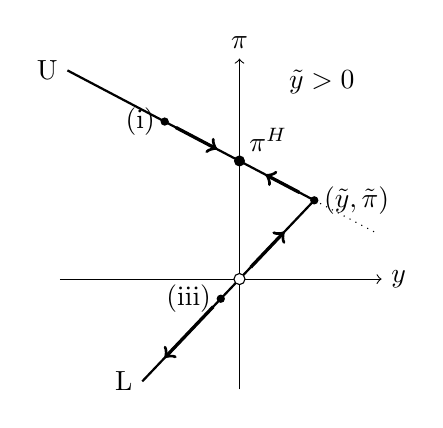
\begin{tikzpicture}[x=0.95cm,y=0.5cm]
  \draw[->] (-2.4,0)--(1.9,0) node[right]{$y$};
  \draw[->] (0,-2.8)--(0,5.6) node[above]{$\pi$};
  \draw[thick] (-1.3,-2.6)--(1,2)--(-2.3,5.3);
  \draw[dotted] (1,2)--(1.8,1.2);
  \draw[->,very thick] (-0.85,3.85)--(-0.3,3.3);
  \draw[->,very thick] (0.8,2.2)--(0.35,2.65);
  \draw[->,very thick] (0.15,0.3)--(0.6,1.2);
  \draw[->,very thick] (-0.35,-0.7)--(-1,-2);
  \fill (0,3) circle (2pt) node[above right]{$\pi^H$};
  \draw[fill=white] (0,0) circle (2pt);
  \fill (1,2) circle (1.5pt) node[right]{$(\tilde y,\tilde\pi)$};
  \fill (-1,4) circle (1.5pt) node[left]{(i)};
  \fill (-0.25,-0.5) circle (1.5pt) node[left]{(iii)};
  \node[left] at (-2.3,5.3){U}; \node[left] at (-1.3,-2.6){L};
  \node at (1.1,5){$\tilde y>0$};
\end{tikzpicture}\qquad
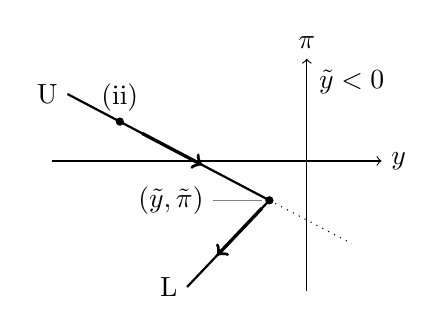
\begin{tikzpicture}[x=0.95cm,y=0.5cm]
  \draw[->] (-3.4,0)--(1,0) node[right]{$y$};
  \draw[->] (0,-3.3)--(0,2.6) node[above]{$\pi$};
  \draw[thick] (-1.6,-3.2)--(-0.5,-1)--(-3.2,1.7);
  \draw[dotted] (-0.5,-1)--(0.6,-2.1);
  \draw[->,very thick] (-2.2,0.7)--(-1.4,-0.1);
  \draw[->,very thick] (-0.6,-1.2)--(-1.2,-2.4);
  \fill (-0.5,-1) circle (1.5pt);
  \draw[gray] (-0.6,-1)--(-1.25,-1) node[left,black]{$(\tilde y,\tilde\pi)$};
  \fill (-2.5,1) circle (1.5pt) node[above]{(ii)};
  \node[left] at (-3.2,1.7){U}; \node[left] at (-1.6,-3.2){L};
  \node at (0.6,2){$\tilde y<0$};
\end{tikzpicture}\par\smallskip
{\small AD curves for the linear rule (dotted: where the rule alone would put AD without the zero bound).
Motion along AD follows $\dot\pi=\lambda y$: down where $y<0$, up where $y>0$. Filled dot: the stable
steady state $\pi^H$; open dot: the unstable trap $\pi=y=i=0$. Starting points of cases (i)--(iii) marked.}
\end{minipage}\end{center}

\parte{b}
\passo{A phase line on the AD curve}{Inflation is predetermined ($\dot\pi$ is finite, so $\pi$ cannot jump), while $y$ moves instantly to keep the economy on the AD curve. So $y(t)=A(\pi(t))$ and the model reduces to one autonomous equation,
\[ \dot\pi=F(\pi)\equiv\lambda A(\pi). \]
$F$ is continuous and piecewise $C^1$, hence locally Lipschitz: the solution is unique, $\pi$ moves monotonically, and it never crosses a zero of $F$. The zeros are the steady states, $A(\pi)=0$: on (L), $\pi/\theta=0$ gives $\pi=0$, admissible iff $0\le\tilde\pi$, i.e.\ $\tilde y\ge0$; on (U), $Y(\pi)=0$ means $r(0,\pi)=0$, i.e.\ $\pi=\pi^H$, admissible iff $\pi^H\ge\tilde\pi$, which requires $\tilde y=Y(\tilde\pi)\ge0$ because $Y$ is decreasing.}
\passo{A trap no interest-rate rule can escape}{Since $\theta y=\min[\pi,-r]\le\pi$, every $\pi<0$ gives $y\le\pi/\theta<0$ and $\dot\pi<0$, \emph{whatever the rule}: with $i\ge0$ the real rate is at least $-\pi>0$.}
\passo{Steady states and stability}{If $\tilde y>0$ and $Y$ turns negative at high inflation (true for the linear rule, and implied by the data of case (i)), there are two steady states, $0<\tilde\pi<\pi^H$, the last inequality because $Y(\tilde\pi)=\tilde y>0=Y(\pi^H)$ with $Y$ decreasing. $F<0$ on $(-\infty,0)$; $F>0$ on $(0,\pi^H)$, because $A=\pi/\theta>0$ on $(0,\tilde\pi]$ and $A=Y>0$ on $[\tilde\pi,\pi^H)$; and $F<0$ on $(\pi^H,\infty)$. So $\pi^H$ is stable with basin $(0,\infty)$, while the liquidity-trap steady state $\pi=y=i=0$ is unstable; locally, $F'(\pi^H)=-\lambda r_2/(\theta+r_1)<0<F'(0)=\lambda/\theta$. If $\tilde y<0$, $A(\pi)\le\tilde y<0$ for every $\pi$ and there is no steady state at all. (At $\tilde y=0$ the two merge at the kink, which attracts from above and repels from below.)}
\passo{Case (i): $\tilde y>0$, $\pi(0)>\tilde\pi$, $y(0)<0$}{The economy starts on (U) with $Y(\pi(0))<0<\tilde y=Y(\tilde\pi)$, so $\pi^H\in(\tilde\pi,\pi(0))$ by continuity and monotonicity of $Y$. On $(\pi^H,\infty)$, $F<0$: inflation falls monotonically, cannot cross $\pi^H$ and, being bounded below, converges to a zero of $F$, which can only be $\pi^H$. Output $y=Y(\pi)$ rises monotonically to $0$, and the nominal rate stays positive throughout because $\pi>\tilde\pi$: an ordinary disinflation, in which the bank cuts the real rate as inflation falls. Near $\pi^H$ the gap decays at rate $\lambda r_2/(\theta+r_1)$; with the linear rule, $Y(\pi)=-b(\pi-\pi^H)/(\theta+a)$, so exactly $\pi(t)=\pi^H+(\pi(0)-\pi^H)e^{-\mu t}$ and $y(t)=y(0)e^{-\mu t}$, with $\mu=\lambda b/(\theta+a)$.}
\passo{Case (ii): $\tilde y<0$, $\pi(0)>\tilde\pi$}{Here $y(0)=Y(\pi(0))\le\tilde y<0$. \emph{Phase 1, on (U).} $\dot\pi=\lambda Y(\pi)\le\lambda\tilde y<0$, so inflation falls at least at speed $\lambda|\tilde y|$ and reaches $\tilde\pi$ at some $t_1\le(\pi(0)-\tilde\pi)/(\lambda|\tilde y|)$, while output $Y(\pi)$ \emph{rises} toward $\tilde y$ because the bank keeps cutting $i$. \emph{Phase 2, on (L), $t\ge t_1$.} Now $i=0$, $y=\pi/\theta$ and $\dot\pi=(\lambda/\theta)\pi$ with $\pi(t_1)=\tilde\pi=\theta\tilde y<0$, so
\[ \pi(t)=\tilde\pi\,e^{(\lambda/\theta)(t-t_1)}\to-\infty,\qquad y(t)=\tilde y\,e^{(\lambda/\theta)(t-t_1)}\to-\infty . \]
Inflation falls for ever; output first recovers, then collapses. With the linear rule, phase 1 is case (i)'s formula aimed at the unreachable $\pi^H=-c/b<\tilde\pi$, so $t_1=\mu^{-1}\ln[(\pi(0)-\pi^H)/(\tilde\pi-\pi^H)]$.}
\passo{Case (iii): $\tilde y>0$, $\pi(0)<\tilde\pi$, $y(0)<0$}{The economy starts on (L), so $y(0)=\pi(0)/\theta<0$ forces $\pi(0)<0$: it starts below the unstable steady state. For all $t$, $\dot\pi=(\lambda/\theta)\pi$, hence $\pi(t)=\pi(0)e^{(\lambda/\theta)t}$ and $y(t)=\pi(t)/\theta$, both falling without bound with $i=0$ throughout; $\pi^H$ exists but is never reached. Had $0<\pi(0)<\tilde\pi$ (so $y(0)>0$), inflation would have risen, crossed $\tilde\pi$ in finite time and converged to $\pi^H$ along (U): $\pi=0$ is the watershed between recovery and collapse.}

\begin{center}\begin{minipage}{\linewidth}\centering
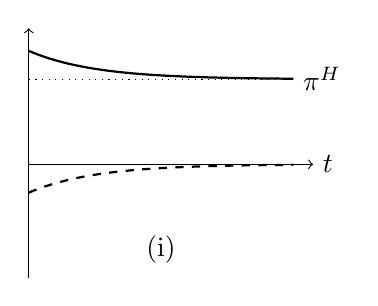
\begin{tikzpicture}[x=0.42cm,y=0.36cm]
  \draw[->] (0,0)--(8.6,0) node[right]{$t$}; \draw[->] (0,-4)--(0,4.8);
  \draw[dotted] (0,3)--(8,3) node[right]{$\pi^H$};
  \draw[thick,domain=0:8,samples=50] plot (\x,{3+exp(-0.5*\x)});
  \draw[thick,dashed,domain=0:8,samples=50] plot (\x,{-exp(-0.5*\x)});
  \node at (4,-3){(i)};
\end{tikzpicture}\quad
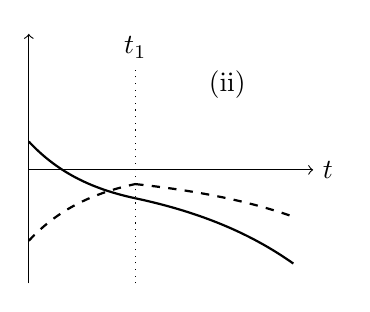
\begin{tikzpicture}[x=0.42cm,y=0.36cm]
  \draw[->] (0,0)--(8.6,0) node[right]{$t$}; \draw[->] (0,-4)--(0,4.8);
  \draw[dotted] (3.2189,-4)--(3.2189,3.6) node[above]{$t_1$};
  \draw[thick,domain=0:3.2189,samples=40] plot (\x,{-1.5+2.5*exp(-0.5*\x)});
  \draw[thick,domain=3.2189:8,samples=40] plot (\x,{-exp(0.25*(\x-3.2189))});
  \draw[thick,dashed,domain=0:3.2189,samples=40] plot (\x,{-2.5*exp(-0.5*\x)});
  \draw[thick,dashed,domain=3.2189:8,samples=40] plot (\x,{-0.5*exp(0.25*(\x-3.2189))});
  \node at (6,3){(ii)};
\end{tikzpicture}\quad
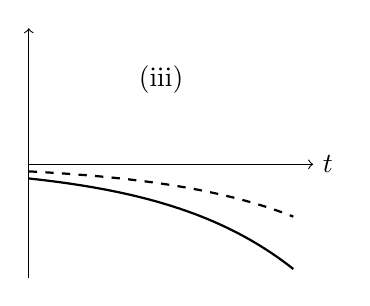
\begin{tikzpicture}[x=0.42cm,y=0.36cm]
  \draw[->] (0,0)--(8.6,0) node[right]{$t$}; \draw[->] (0,-4)--(0,4.8);
  \draw[thick,domain=0:8,samples=50] plot (\x,{-0.5*exp(0.25*\x)});
  \draw[thick,dashed,domain=0:8,samples=50] plot (\x,{-0.25*exp(0.25*\x)});
  \node at (4,3){(iii)};
\end{tikzpicture}\par\smallskip
{\small Time paths for the linear rule: $\pi(t)$ solid, $y(t)$ dashed. (i) $c=-9$, $\pi(0)=4$, so
$\pi^H=3$ and $\mu=\frac12$; (ii) $c=4.5$, $\pi(0)=1$, $t_1=2\ln5\approx3.22$; (iii) $c=-9$, $\pi(0)=-\frac12$.}
\end{minipage}\end{center}

\passo{The way out: raise expected inflation}{Suppose the bank can make expected inflation exceed current inflation by $\Delta>0$ through a credible promise of higher future prices. The real rate in the IS curve becomes $i-\pi-\Delta$, the rule still targets it, $i=\max[0,\pi+\Delta+r(y,\pi)]$, and the first step of (a) now gives
\[ \theta y=\min\bigl[\pi+\Delta,\ -r(y,\pi)\bigr]. \]
Branch (U) is unchanged, but (L) shifts out to $y=(\pi+\Delta)/\theta$: the repelling point moves from $\pi=0$ to $\pi=-\Delta$, and any $\pi>-\Delta$ on (L) now has $y>0$ and $\dot\pi>0$. In case (iii), a promise $\Delta>-\pi(t)$ turns the spiral into a recovery at $i=0$ without touching $r(\cdot)$, and it need only last until $\pi>0$, when the economy has entered the basin $(0,\infty)$ of $\pi^H$. In case (ii) no temporary promise is enough, since $A<0$ at every $\pi$: the rule's own steady state, if any, needs $i<0$. What works there is a permanently higher target, $\pi^H>0$ (with a natural rate, $\pi^H>-r^n$), which moves the kink to $\tilde y>0$ and creates the basin of recovery, plus a temporary $\Delta$ if inflation is already negative.}

\intuicao{Above $\tilde\pi$ the rule is stabilising: lower inflation brings a lower real rate, higher output and, through $\dot\pi=\lambda y$, an end to disinflation. Below $\tilde\pi$ the nominal rate is stuck at zero and the real rate is $-\pi$, so the feedback changes sign: lower inflation raises the real rate, depresses output and lowers inflation further. This deflationary spiral is why $\pi=0$ is a steady state that repels, and why the rule $r(\cdot)$, however aggressive, is powerless on (L). The lever left is the wedge between expected and current inflation, which is Benigno's (2015, \S9) point: in his AD equation (21) the real rate is $i-(\bar p-p)$, so raising the long-run price level $\bar p$ lowers it even at $i=0$ and shifts both AD and its zero-bound version AD$_0$ outward. In Romer's model expected inflation is tied to current inflation, and $\Delta$ is exactly the missing $\bar p$ channel.}
\armadilha{(1) Drawing the zero-bound branch as a continuation of the downward-sloping AD: below $\tilde\pi$ the AD bends back. (2) Expecting a more aggressive rule to rescue case (iii): on (L) the rule is inoperative, and for $\pi<0$ every rule gives $y\le\pi/\theta<0$. (3) Treating $y(0)$ as a free initial condition: $y$ is pinned by $\pi(0)$ through $A$, so the conditions on $y(0)$ in (i) and (iii) only place $\pi(0)$ relative to $\pi^H$ and $0$. (4) Claiming that output falls monotonically in (ii): it first rises along (U).}
\refbib{Romer (2012), \S6.4 (pp.~255--267): eqs.~(6.22)--(6.23), the rule (6.26) and Figures 6.8--6.9; \S11.6 on the zero lower bound. Benigno (2015), \S9 (``Liquidity trap'') and the AD equation (21), p.~509. Krugman (1998), cited there.}
\checado{\texttt{check-6-10-6-7.py} confirms the identity $\pi-\max[0,\pi+r]=\min[\pi,-r]$, solves the AD equation by bisection and matches the piecewise $A(\pi)$ (kink $(1,2)$ and $\pi^H=3$ for $c=-9$; kink $(-0.5,-1)$ for $c=4.5$), confirms the branch split at $\tilde\pi$ and the slope $-(\theta+r_1)/r_2$ on a nonlinear rule, checks the kink formulas with $r^n$ and with $\Delta$ in sympy, and integrates $\dot\pi=\lambda A(\pi)$ by RK4: (i) converges to $\pi^H$ along the closed form, (ii) crosses $\tilde\pi$ at $t_1=2\ln5$ with peak output $\tilde y$ and then diverges, (iii) diverges, $\pi(0)=0.1$ recovers, no linear rule tried escapes from $\pi<0$, and a temporary $\Delta=1$ rescues case (iii) while $\Delta=0.3$ does not. The solution manual agrees on (a) and all three cases (it works in $(y,r)$ space); it does not discuss the steady state at $\pi=0$ or the way out.}
